%!TEX root = Thesis.tex

\chapter{Clustering}
\label{chapter:clustering}

\section{The problem of clustering}
\label{sec:clustering}

% have to say that I'm using a vectorial representation of the data (data as vector of features) without loss of generality. I have to specify that I'm dealing with a partitioning clustering but other kinds exist. In this context (of vectorial data and partitional algorithms) K-Means is one of the most known algorithms. It's simple and fast and, although it only yields good results in a specific set of cases, it's often used as a starting point for more robust algorithms, e.g. EAC. 

%this is mostly taken from Jain's 50 years beyond K-Means
Hundreds of methods for data analysis exist.
Many of these methods fall into the realm of machine learning, which is usually divided into 2 major groups: \textit{supervised} and \textit{unsupervised} learning.
% TODO: add some reference for the 2 major groups; optional: explain what learning is
Supervised learning deals with labeled data, i.e. data for which ground truth is known, and tries to solve the problem of classification.
Examples of supervised learning algorithms are Neural Networks, Decision Trees, Linear Regression and Support Vector Machines. %TODO add refs
 %TODO: add ref for solving classification
Unsupervised learning deals with unlabeled data for which no extra information is known
Clustering algorithms, expectation-maximization and Principal Component Analysis are examples of unsupervised algorithms. % TODO: add refs

Cluster analysis methods are unsupervised and the backbone of the present work.
The goal of data clustering, as defined by \cite{Jain2010}, is the discovery of the \textit{natural grouping(s)} of a set of patterns, points or objects.
In other words, the goal of data clustering is to discover structure on data.
The methodology used is to group patterns (usually represented as a vector of measurements or a point in space \cite{Jain1999}) based on some similarity, such that patterns belonging to the same cluster are typically more similar to each other than to patterns of other clusters.
Clustering is a strictly data-driven method, in contrast with classification techniques which have a training set with the desired labels for a limited collection of patterns.
Because there is very little information, as few assumptions as possible should be made about the structure of the data (e.g. number of clusters).
And, because clustering typically makes as few assumptions on the data as possible, it is appropriate to use it on exploratory structural analysis of the data.
The process of clustering data has three main stages \cite{Jain1999}:

\begin{itemize}
    \item \textbf{Pattern representation} refers to the choice of representation of the input data in terms of size, scale and type of features.
    The input patterns may be fed directly to the algorithms or undergo \emph{feature selection} and/or \emph{feature extraction}. The former is simply the selection of which features of the originally available should be used.
    The later is deals with the transformation of the original features such that the resulting features will produce more accurate and insightful clusterings, e.g. Principal Component Analysis.
    It should be noted that 
    \item \textbf{Pattern similarity} refers to the definition of a measure for computing the similarity between two patterns.
    \item \textbf{Grouping} refers to the algorithm that will perform the actual clustering on the dataset with the defined pattern representation, using the appropriate similarity measure.
\end{itemize}

As an example, Figure \ref{fig:intro raw} shows the plot of a simple synthetic dataset - a Gaussian mixture of 5 distributions.
No extra information other than the position of the points is given, since clustering algorithms are unsupervised methods.
Figure \ref{fig:intro natural} presents the desired clustering for this given dataset.

% Part of this went to the K-Means section
% The number of clusters was purposefully set to an "incorrect" number to demonstrate that the number of cluster of a dataset is not trivial to discover, even in such a simple example.
% In this synthetic dataset, the number of clusters is not clear due to the two superimposed Gaussians.
% The number of clusters is a common initialization parameter for clustering methods.
% When no prior information about the dataset is given, the number of clusters can be hard to discover.

\begin{figure}[!ht]
    \centering
    \begin{subfigure}[b]{0.45\textwidth}
        \centering
        \includegraphics[width=\textwidth]{introduction/img/cluster_example_raw}
        \caption{Input data, unlabeled.}
        \label{fig:intro raw}
    \end{subfigure}
    %\hfill
    \begin{subfigure}[b]{0.45\textwidth}
        \centering
        \includegraphics[width=\textwidth]{introduction/img/cluster_example_natural}
        \caption{Desired labels.}
        \label{fig:intro natural}
    \end{subfigure}

    \caption{Gaussian mixture of 5 distributions. Fig. \ref{fig:intro raw} shows the raw input data, i.e. how the algorithms "see" the data. Fig. \ref{fig:intro natural} shows the desired labels for each point, which here means their corresponding Gaussian.}
    \label{fig:clustering plots}
\end{figure}


\section{Definitions and Notation}

This section will introduce relevant definitions and notation within the clustering context that will be used throughout the rest of this document.

% TODO: review this part of the vector notation, it's fishy right now
%pattern, features
A \emph{pattern} $\mathbf{x}$ is a single data item and, without loss of generalization, it consists of a set of $d$ \emph{features} $x_i$ that characterize that data item, $\mathbf{x} = (x_1, \ldots, x_d)$, where $d$ is referred to as the dimensionality of the pattern.
%pattern set
A \emph{pattern set} (or data set) $\mathcal{X}$ is then the collection of all $n$ patterns $\mathcal{X} = \{ \mathbf{x}_1, \ldots, \mathbf{x}_n \}$.
The number of features is usually the same for all patterns in a given pattern set.

%classes
In cluster analysis, the desired clustering, typically, is one that reflects the natural structure of the data, i.e. the original true clustering.
In other words, one wants to group the patterns that came from the same state of nature when they were generated, the same \emph{class}.
A class, then, can be viewed as a source of patterns and the effort of the clustering algorithm is to group patterns from the same source.
Throughout this work, these classes will be also be referred to as the "natural" or "true" clusterings.
%labels
\emph{Hard} clustering (or partitional) techniques assign a class label $l_i$ to each pattern $\mathbf{x}_i$.
The whole set of labels of a pattern set $\mathcal{X}$ is given by $\mathcal{L} = {l_1, \ldots, l_n}$.
%partition
% Throughout this document, the whole set of labels may also be referred to as a partition.
Closely related to the whole set of labels is the concept of a \emph{partition}, which completely describes a clustering in a different way.
A partition $P$ is a collection of $k$ \emph{clusters}.
A cluster $C$ is a subset of $nc$ patterns $\mathbf{x}_i$ taken from the pattern set, where the patterns belonging to one subset don't belong to any other in the same partition.
A clustering \emph{ensemble} $\mathbb{P}$ is a set of partitions from a given pattern set.
The relationship between the above concepts is condensed in the following expressions:

\begin{align}
    \mathbb{P} &= \left \{   P^1, P^2, \ldots P^N   \right \}  \label{eq:ensemble} \\
    P^j &= \left \{   C^j_1, C^j_2, \ldots C^{j}_{k_j}   \right \}  \label{eq:partition} \\
    C^j_i &= \left \{   x_1, x_2, \ldots x_{nc^j_i}   \right \} \label{eq:cluster}
\end{align}


%similarity
Finally, a \emph{similarity measure} is a way of quantifying how similar two patterns are in the feature space, usually using a metric such as Euclidean distance.


\section{Characteristics of clustering techniques}

Clustering algorithms may be described according to different properties.
For the sake of completeness, a small discussion of some properties will be layed out in this section.

% hierarchical: agglomerative vs divisive
A clustering algorithm is considered hierarchical if it produces a clustering structure presenting 

%clustering techniques


There are two big main types of clustering: hierarchical and partitional.

usually some metric (e.g. euclidean distance, Pearson correlation). %TODO reference for a method for both euclidean distance and Pearson correlation






Cluster analysis is a relevant technique across several domains (\cite{Aggarwal2014}):

\begin{itemize}
	\item grouping users with similar behaviour or preferences in \textbf{customer segmentation};
	\item image segmentation in the field of \textbf{image processing};
	\item clustering gene expression data, among other application, in the domain of \textbf{biological data analysis};
	\item generation of hierarchical structure for easy access and retrieval of \textbf{information systems}; % not referenced in book
\end{itemize}

% Clustering is used in a wide variety of fields to solve numerous problems, e.g.:
% %TODO provide references to all of this
% % see https://sites.google.com/site/dataclusteringalgorithms/clustering-algorithm-applications
% % has applications with articles
% \begin{itemize}
% \item image segmentation in the field of image processing;
% \item generation of hierarchical structure for easy access and retrieval of information systems;
% \item recommender systems by grouping users by their behaviour and/or preferences;
% \item clustering customers for targeted marketing in 
% \item clustering gene expression data in biology;
% \item grouping of 
% \end{itemize}



\section{K-Means}

K-Means is one of the earliest clustering algorithms to offer a partitional solution to the clustering problem

It's also widely used due to it's simplicity and efficiency.
Because of this, it's also often used as a foundational step of more complex and robust algorithms, such as EAC.
 the algorithm works as follows

explain K-means algorithm

As an example, the output of the K-means algorithm to the data presented in Fig. \ref{fig:clustering plots} is represented in Fig. \ref{fig:intro kmeans}.
The algorithm executed with 4 random centroids.

\begin{figure}[hbtp]
\centering
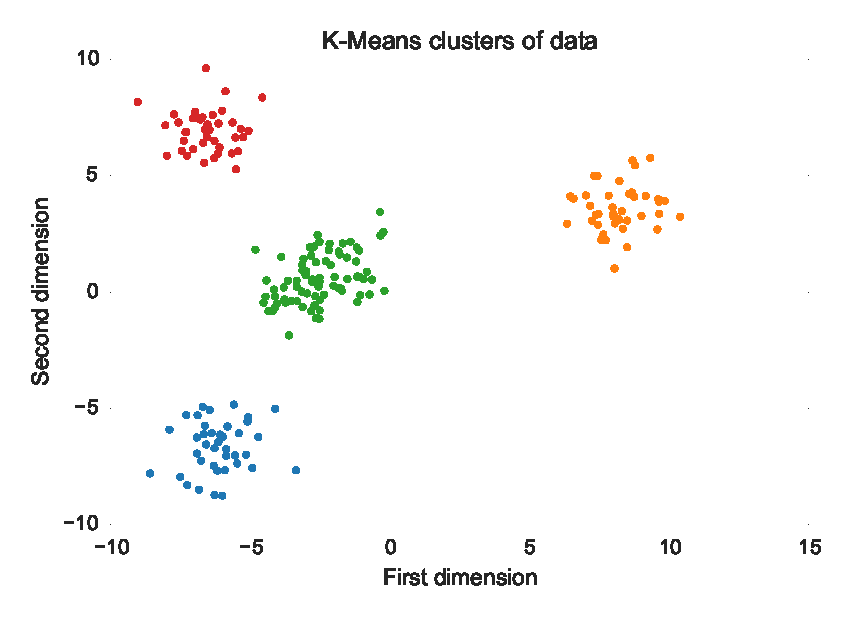
\includegraphics[width=0.5\textwidth]{introduction/img/cluster_example_kmeans}
\caption{The output labels of the K-Means algorithm with the number of clusters (input parameter) set to 4.}
\label{fig:intro kmeans}\end{figure}

The number of clusters was purposefully set to an "incorrect" number to demonstrate that it is not trivial to discover, even in such a simple example.
In this synthetic dataset, the number of clusters is not clear due to the two superimposed Gaussians.
When no prior information about the dataset is given, the number of clusters can be hard to discover.
This is why, when available, a domain expert may provide valuable insight on tuning the initialization parameters.

\section{Single-Link}

Do the same thing as K-Means but for SL